\section{\LaTeX}

{\setbeamertemplate{background canvas}{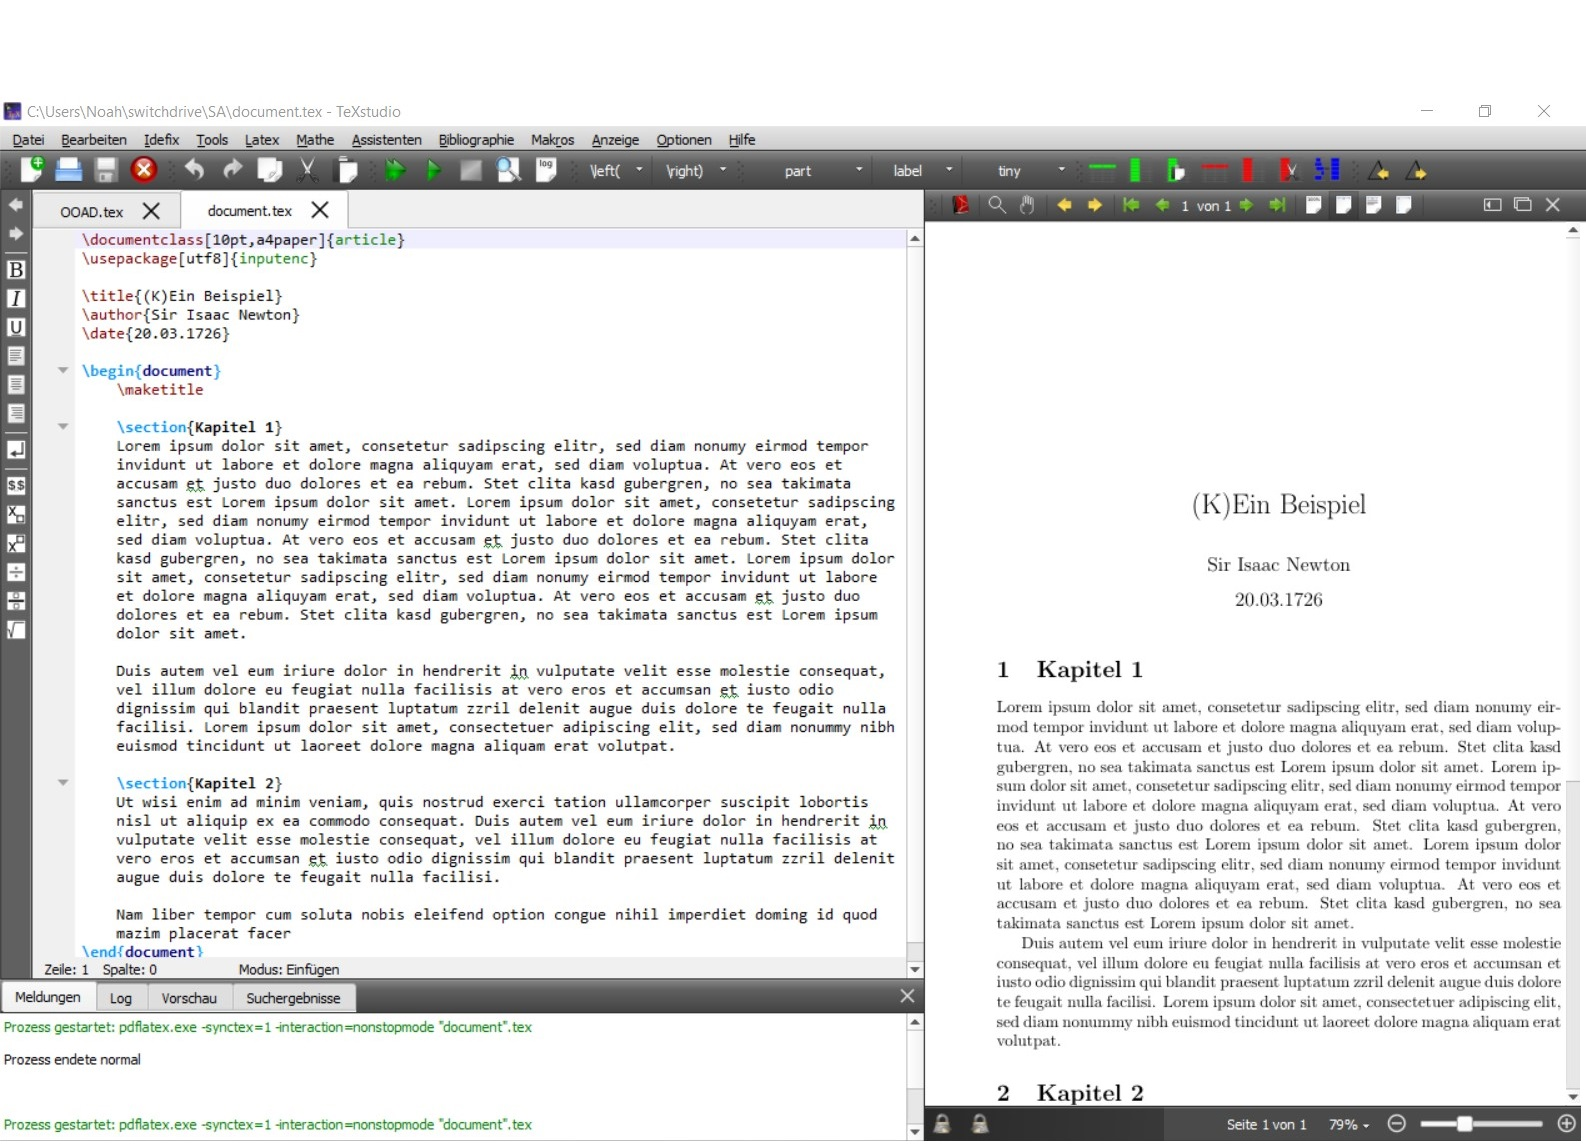
\includegraphics[width=\paperwidth]{pic/bild}}
\begin{frame}

\end{frame}
}

\begin{frame}
	\begin{itemize}
		\item \LaTeX: \textbf{La}mport \textbf{TeX} 
		\item TeX: Textsatzsystem 
		\item Kein WYSIWYG sondern WYSIWYAF
	\end{itemize}
\end{frame}

\begin{frame}{Warum \LaTeX?}
\begin{itemize}
	\item Open-Source 
	\item Grosse Community 
	\item Performance 
	\item Kein WYSIWYG 
	\item Professionell 
	\item Wissenschaftliche Formeln 
	\item Cross-Platform
\end{itemize}
\end{frame}
